%!TEX TS-program = xelatex
%!TEX encoding = UTF-8 Unicode

% Author: Romain "Artefact2" Dal Maso <artefact2@gmail.com>
% 
% This program is free software. It comes without any warranty, to the
% extent permitted by applicable law. You can redistribute it and/or
% modify it under the terms of the Do What The Fuck You Want To Public
% License, Version 2, as published by Sam Hocevar. See
% http://sam.zoy.org/wtfpl/COPYING for more details.

\newlength{\phNoteCurparskip}
\newlength{\phNoteCurparindent}
\newlength{\phNotePrevSubsubsectionSkip}
\newlength{\phNotePrevParagraphSkip}
\newlength{\phNoteBW}
\newlength{\phNoteBH}
\newlength{\phNoteRW}
\newlength{\phNotePS}
\newlength{\phNotePadding}
\newlength{\phNoteBoxWidth}
\newlength{\phNoteBoxHeight}
\newlength{\phNoteBoxDepth}
\newsavebox{\phNoteBox}

\setlength{\phNoteBW}{1pt} % Border width for note
\setlength{\phNoteBH}{6pt} % Border height for note
\setlength{\phNoteRW}{1pt} % Rule width for note2
\setlength{\phNotePS}{3pt} % Point corner for note2
\setlength{\phNotePadding}{2pt} % Horizontal padding inside notes

\newcommand*{\phNotePrevSubsubsectionStyle}{}
\newcommand*{\phNotePrevParagraphStyle}{}

\newcommand*{\phNoteBefore}{%
  \setlength{\phNoteCurparskip}{\parskip}%
  \setlength{\phNoteCurparindent}{\parindent}%
  \renewcommand*{\phNotePrevSubsubsectionStyle}{\subsubsecheadstyle}%
  \renewcommand*{\phNotePrevParagraphStyle}{\paraheadstyle}%
  \setlength{\phNotePrevSubsubsectionSkip}{\beforesubsubsecskip}%
  \setlength{\phNotePrevParagraphSkip}{\beforeparaskip}%
  \setsubsubsecheadstyle{\scaly\large\bfseries\scshape}%
  \setparaheadstyle{\scaly\bfseries}%
  \setbeforesubsubsecskip{0pt}%
  \setbeforeparaskip{0pt}%
}

\newcommand*{\phNoteAfter}{%
  \setsubsubsecheadstyle{\phNotePrevSubsubsectionStyle}%
  \setparaheadstyle{\phNotePrevParagraphStyle}%
  \setbeforesubsubsecskip{\phNotePrevSubsubsectionSkip}%
  \setbeforeparaskip{\phNotePrevParagraphSkip}%
}

% XXX where is that 1pt vertical offset FROM?!
\newcommand*{\phNoteDraw}{%
  \settowidth{\phNoteBoxWidth}{\usebox{\phNoteBox}}%
  \settoheight{\phNoteBoxHeight}{\usebox{\phNoteBox}}%
  \settodepth{\phNoteBoxDepth}{\usebox{\phNoteBox}}%
  \TPoptions{absolute=false}%
  \noindent\vspace*{\phNoteBH}\hspace*{\phNoteBW}%
  \begin{textblock*}{\linewidth}(0pt,-\phNoteBH+1pt)
    \scalebox{1}[-1]{\includegraphics[width=1.307\phNoteBH,height=\phNoteBH]{assets/note-corner}}
  \end{textblock*}%
  \begin{textblock*}{\linewidth}(\phNoteBoxWidth-1.307\phNoteBH,-\phNoteBH+1pt)
    \scalebox{-1}[-1]{\includegraphics[width=1.307\phNoteBH,height=\phNoteBH]{assets/note-corner}}
  \end{textblock*}%
  \begin{textblock*}{\linewidth}(0pt,\phNoteBoxHeight+\phNoteBoxDepth+1pt)
    \scalebox{1}[1]{\includegraphics[width=1.307\phNoteBH,height=\phNoteBH]{assets/note-corner}}
  \end{textblock*}%
  \begin{textblock*}{\linewidth}(\phNoteBoxWidth-1.307\phNoteBH,\phNoteBoxHeight+\phNoteBoxDepth+1pt)
    \scalebox{-1}[1]{\includegraphics[width=1.307\phNoteBH,height=\phNoteBH]{assets/note-corner}}
  \end{textblock*}%
  \begin{textblock*}{\linewidth}(1.306\phNoteBH,-\phNoteBH+1pt)
    \scalebox{1}[-1]{\includegraphics[width=\phNoteBoxWidth-2.612\phNoteBH,height=\phNoteBH]{assets/note-bottom}}
  \end{textblock*}%
  \begin{textblock*}{\linewidth}(1.306\phNoteBH,\phNoteBoxHeight+\phNoteBoxDepth+1pt)
    \includegraphics[width=\phNoteBoxWidth-2.612\phNoteBH,height=\phNoteBH]{assets/note-bottom}
  \end{textblock*}%
  \begin{textblock*}{\linewidth}(-\phNoteBW,1pt)
    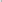
\includegraphics[width=\phNoteBW,height=\phNoteBoxHeight+\phNoteBoxDepth]{assets/note-side}
  \end{textblock*}%
  \begin{textblock*}{\linewidth}(\phNoteBoxWidth,1pt)
    \reflectbox{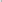
\includegraphics[width=\phNoteBW,height=\phNoteBoxHeight+\phNoteBoxDepth]{assets/note-side}}
  \end{textblock*}%
  \usebox{\phNoteBox}\vspace*{\phNoteBH}%
  \TPoptions{absolute=true}%
}

\NewEnviron{phNote}[1][!ht]{%
\phNoteBefore%
\begin{figure}[#1]%
  \sbox{\phNoteBox}{%
    \colorbox{note}{%
      \hspace*{\phNotePadding}\begin{minipage}[b]{\linewidth-2\phNotePadding-2\phNoteBW-2\fboxsep}%
        \setlength{\parskip}{\phNoteCurparskip}%
        \setlength{\parindent}{\phNoteCurparindent}%
        \noindent\scaly\small\BODY%
      \end{minipage}%
      \hspace*{\phNotePadding}%
    }%
  }%
  \phNoteDraw%
\end{figure}%
\phNoteAfter%
}

\NewEnviron{phNoteWide}[1][t]{%
\phNoteBefore%
\begin{figure*}[#1]%
  \sbox{\phNoteBox}{%
    \colorbox{note}{%
      \hspace*{\phNotePadding}\begin{minipage}[b]{\linewidth-2\phNotePadding-2\phNoteBW-2\fboxsep}%
        \setlength{\parskip}{\phNoteCurparskip}%
        \setlength{\parindent}{\phNoteCurparindent}%
        \noindent\scaly\small\BODY%
      \end{minipage}%
      \hspace*{\phNotePadding}%
    }%
  }%
  \phNoteDraw%
\end{figure*}%
\phNoteAfter%
}

% XXX same
\newcommand*{\phNoteDrawVar}{%
  \settowidth{\phNoteBoxWidth}{\usebox{\phNoteBox}}%
  \settoheight{\phNoteBoxHeight}{\usebox{\phNoteBox}}%
  \settodepth{\phNoteBoxDepth}{\usebox{\phNoteBox}}%
  \TPoptions{absolute=false}%
  \noindent\hspace*{\phNoteRW}%
  \begin{textblock*}{\linewidth}(-.5\phNoteRW,1pt-\phNotePS)
  \includegraphics[width=\phNoteBoxWidth+\phNoteRW,height=\phNotePS]{assets/note-var-top}
  \end{textblock*}%
  \begin{textblock*}{\linewidth}(-.5\phNoteRW,1pt+\phNoteBoxHeight+\phNoteBoxDepth)
  \scalebox{1}[-1]{\includegraphics[width=\phNoteBoxWidth+\phNoteRW,height=\phNotePS]{assets/note-var-top}}
  \end{textblock*}%
  \begin{textblock*}{\phNotePS}(-.5\phNotePS-.5\phNoteRW,1pt-\phNotePS)
  
\includegraphics[width=\phNotePS,height=\phNotePS]{assets/note-var-corner}
  \end{textblock*}%
  \begin{textblock*}{\phNotePS}(\phNoteBoxWidth+.5\phNoteRW-.5\phNotePS,1pt-\phNotePS)
  
\includegraphics[width=\phNotePS,height=\phNotePS]{assets/note-var-corner}
  \end{textblock*}%
  \begin{textblock*}{\phNotePS}(-.5\phNotePS-.5\phNoteRW,1pt+\phNoteBoxHeight+\phNoteBoxDepth)
  
\includegraphics[width=\phNotePS,height=\phNotePS]{assets/note-var-corner}
  \end{textblock*}%
  \begin{textblock*}{\phNotePS}(\phNoteBoxWidth+.5\phNoteRW-.5\phNotePS,1pt+\phNoteBoxHeight+\phNoteBoxDepth)
  
\includegraphics[width=\phNotePS,height=\phNotePS]{assets/note-var-corner}
  \end{textblock*}%
  \begin{textblock*}{\phNoteRW}(-\phNoteRW,1pt-.5\phNotePS)
  {\color{chapter}\rule{\phNoteRW}{\phNoteBoxHeight+\phNoteBoxDepth+\phNotePS}}
  \end{textblock*}%
  \begin{textblock*}{\phNoteRW}(\phNoteBoxWidth,1pt-.5\phNotePS)
  {\color{chapter}\rule{\phNoteRW}{\phNoteBoxHeight+\phNoteBoxDepth+\phNotePS}}
  \end{textblock*}%
  \usebox{\phNoteBox}\hspace*{\phNoteRW}%
  \TPoptions{absolute=true}%
}

\NewEnviron{phNote2}[1][!ht]{%
\phNoteBefore%
\begin{figure}[#1]%
  \sbox{\phNoteBox}{%
    \colorbox{white}{%
      \hspace*{\phNotePadding}\begin{minipage}[b]{\linewidth-2\phNotePadding-2\phNoteRW-2\fboxsep}%
        \setlength{\parskip}{\phNoteCurparskip}%
        \setlength{\parindent}{\phNoteCurparindent}%
        \noindent\scaly\small\BODY%
      \end{minipage}%
      \hspace*{\phNotePadding}%
    }%
  }%
  \phNoteDrawVar%
\end{figure}%
\phNoteAfter%
}

\NewEnviron{phNoteWide2}[1][t]{%
\phNoteBefore%
\begin{figure*}[#1]%
  \sbox{\phNoteBox}{%
    \colorbox{white}{%
      \hspace*{\phNotePadding}\begin{minipage}[b]{\linewidth-2\phNotePadding-2\phNoteRW-2\fboxsep}%
        \setlength{\parskip}{\phNoteCurparskip}%
        \setlength{\parindent}{\phNoteCurparindent}%
        \noindent\scaly\small\BODY%
      \end{minipage}%
      \hspace*{\phNotePadding}%
    }%
  }%
  \phNoteDrawVar%
\end{figure*}%
\phNoteAfter%
}
